\documentclass[a4paper,10pt]{article}
\usepackage[utf8]{inputenc}
\usepackage{graphicx}
\usepackage{listings}
\usepackage{physics}
\usepackage[margin=1in]{geometry}
\usepackage{subcaption}


\lstset{basicstyle=\footnotesize, breaklines = false}

\date{\today}
\title{FYS-MENA4111 - lab report 2}
\author{Mikael B. Kiste}

\begin{document}
  \maketitle
  \tableofcontents
  \newpage
  \section{Introduction}
  In this lab we explore the cut-off energy for simulations. The cut-off limits how long the simulation will run to try and stabilize the structure before settling with the result. A too strong requirement will require a long time to compute but too weak of a requirement will not give accurate results. Therefore a balance is needed (also depending on the parameters in the specific simulation)
	\section{results}
	First we can show a plot of how the absolute values of the energy (comparing a system with completely seperated atoms to that of the actual structure with interatomic forces coming into play through the simulations)
	\begin{figure}[h]
		\begin{center}
		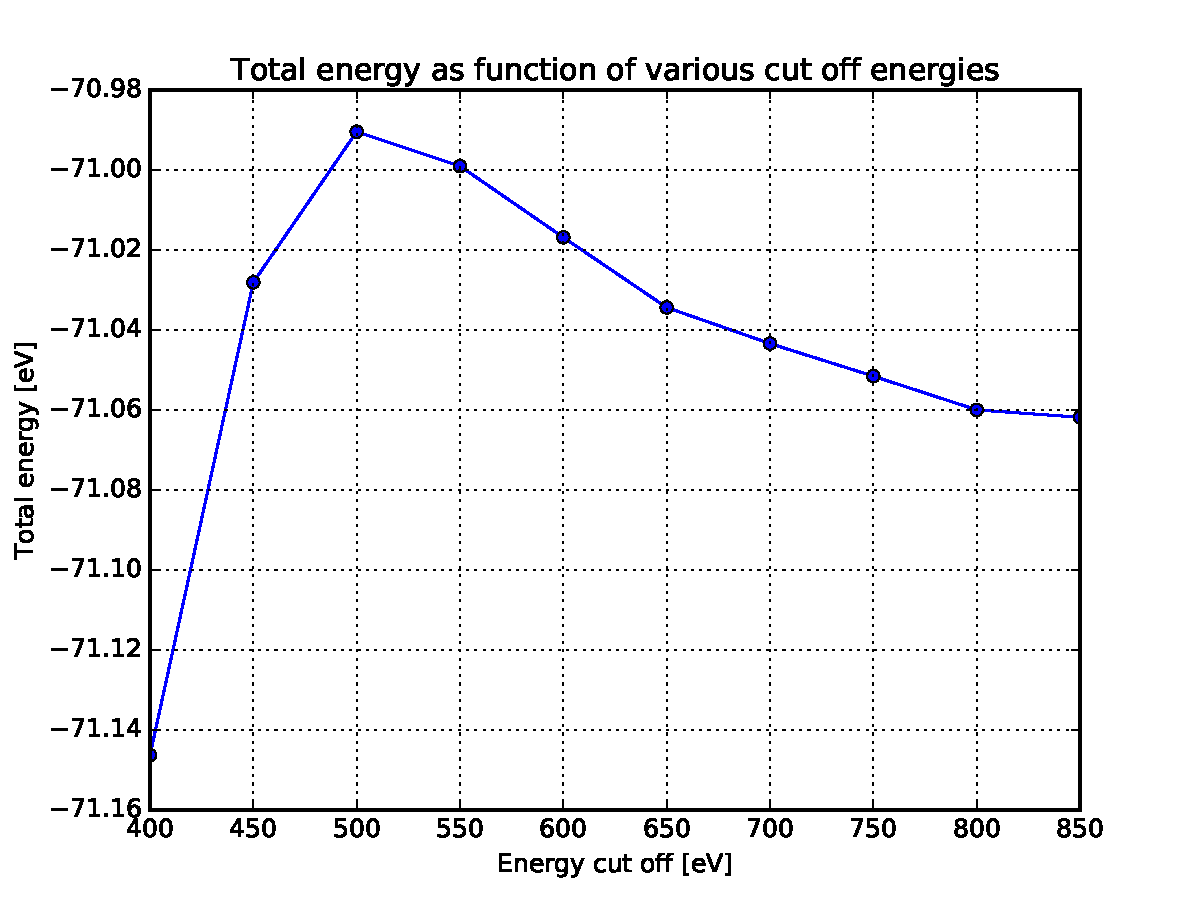
\includegraphics[width=0.9\linewidth]{TOTENplot.pdf}
		\end{center}
	\end{figure}

  \begin{figure}[h]
  	\begin{center}
  		\begin{subfigure}{0.4\textwidth}
  			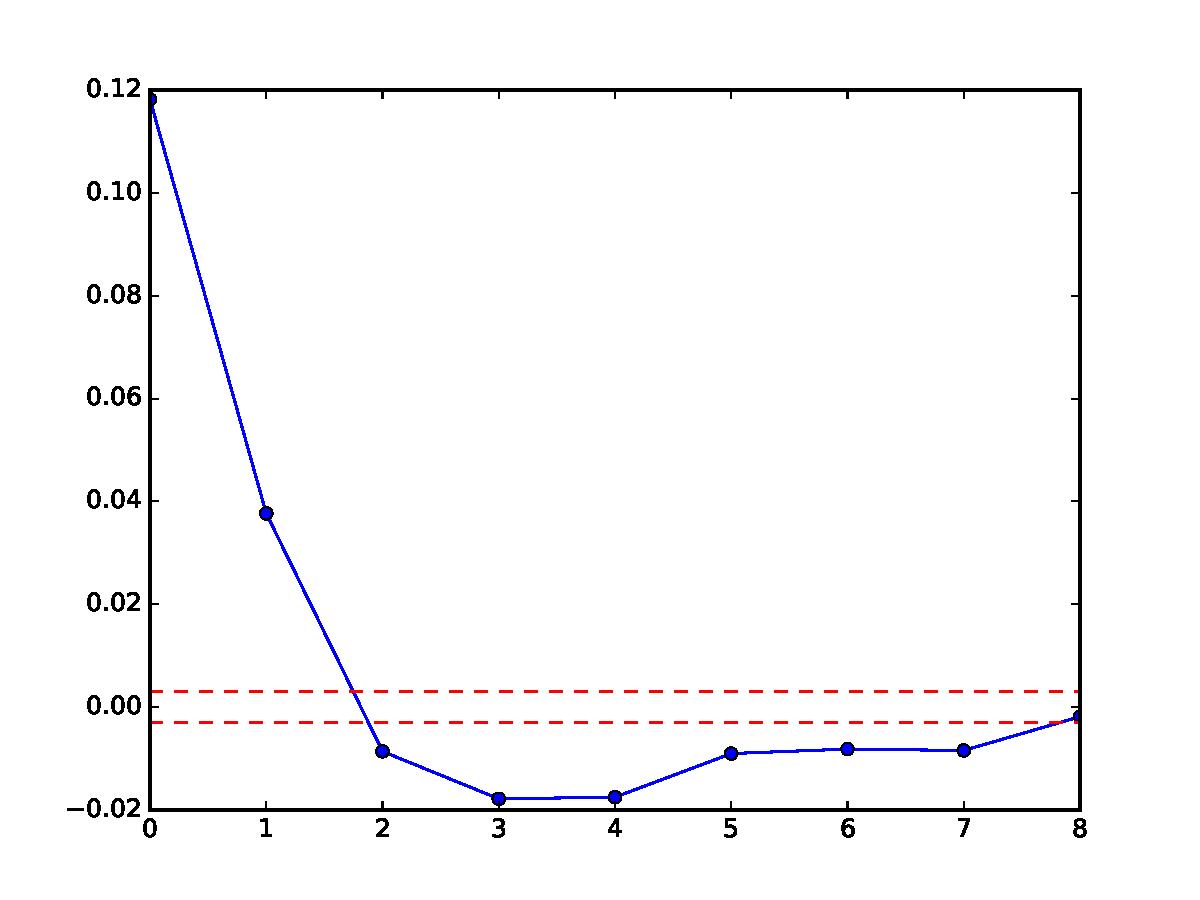
\includegraphics[width=1.0\linewidth]{energyDiff.pdf} 
  			\caption{Difference in the energies in eV}
  			\label{fig:subim1}
  		\end{subfigure}
  		\begin{subfigure}{0.4\textwidth}
  			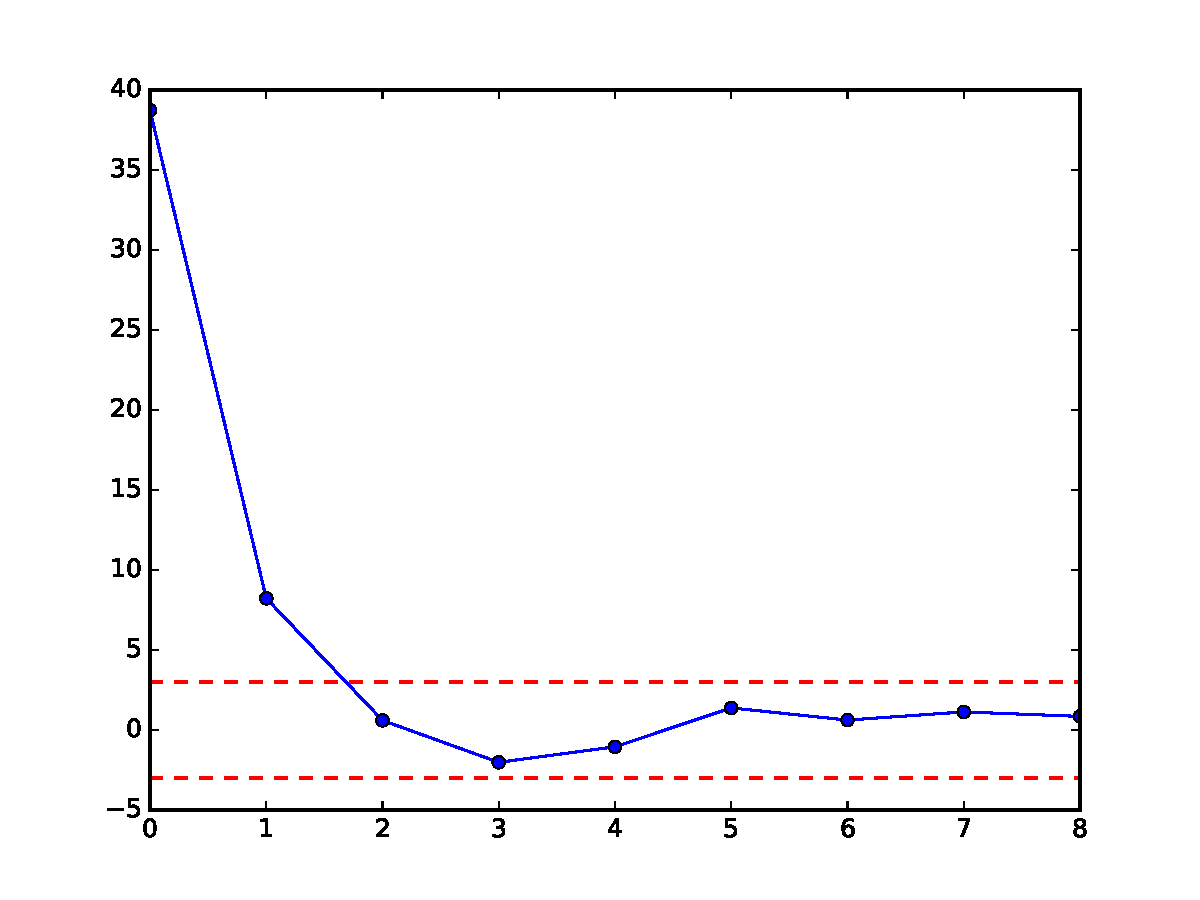
\includegraphics[width=1.0\linewidth]{pressDiff.pdf}
  			\caption{Difference in the pressure in kbar}
  			\label{fig:subim2}
  		\end{subfigure}
  		
  		\caption{Here are plots of the differences in relative energies and pressures simulations with different cut-off limits. The difference is found by comparing two different simulations separated by 50ev in the cut-off. For the energies almost all points lie outside the limit interval, only the last point meets the requirement. For the pressure quite a lot of the points are within the interval}
  		\label{fig:image2}
  	\end{center}
  \end{figure}
	  \begin{figure}[h]
		\begin{center}
			\begin{subfigure}{0.4\textwidth}
				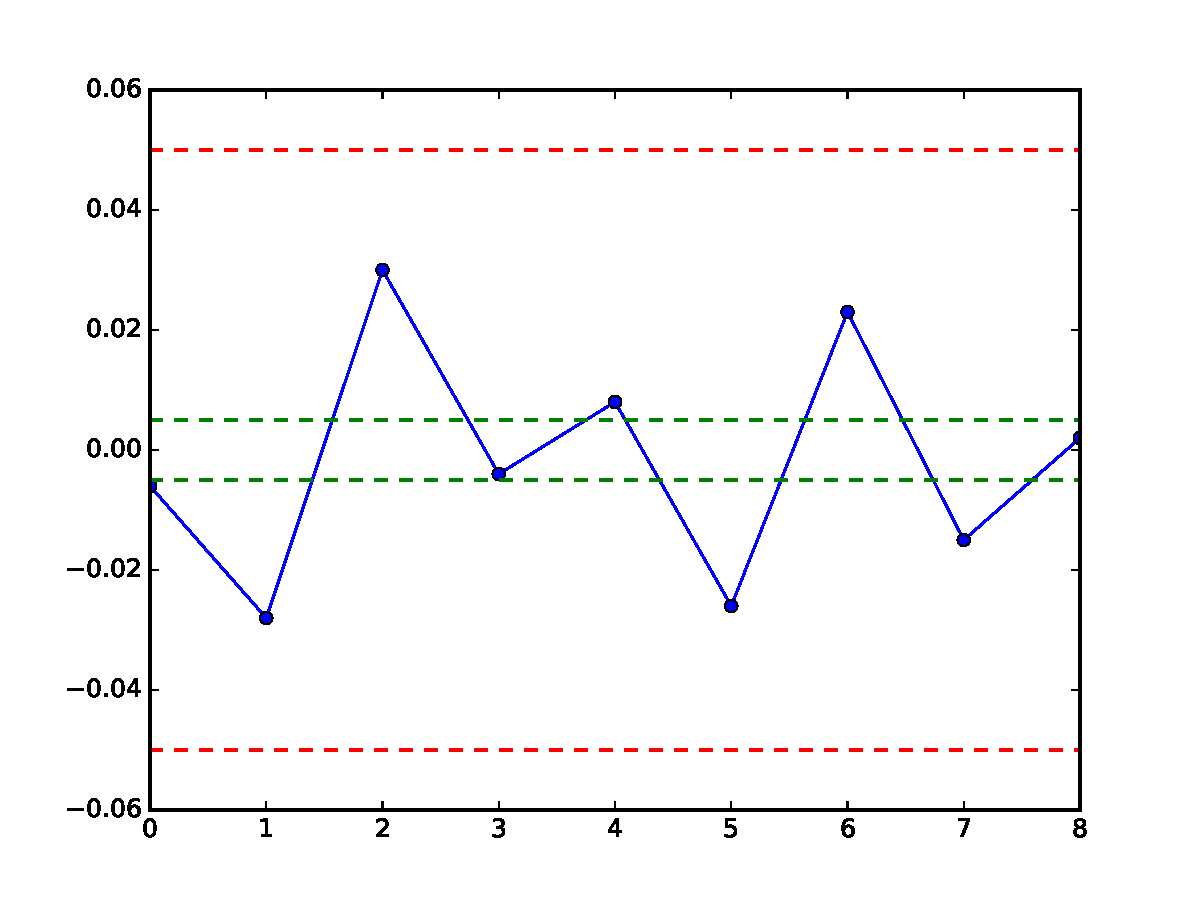
\includegraphics[width=1.0\linewidth]{forceDiff.pdf} 
				\caption{Difference in the force in eV/å}
				\label{fig:subim1}
			\end{subfigure}
			\begin{subfigure}{0.4\textwidth}
				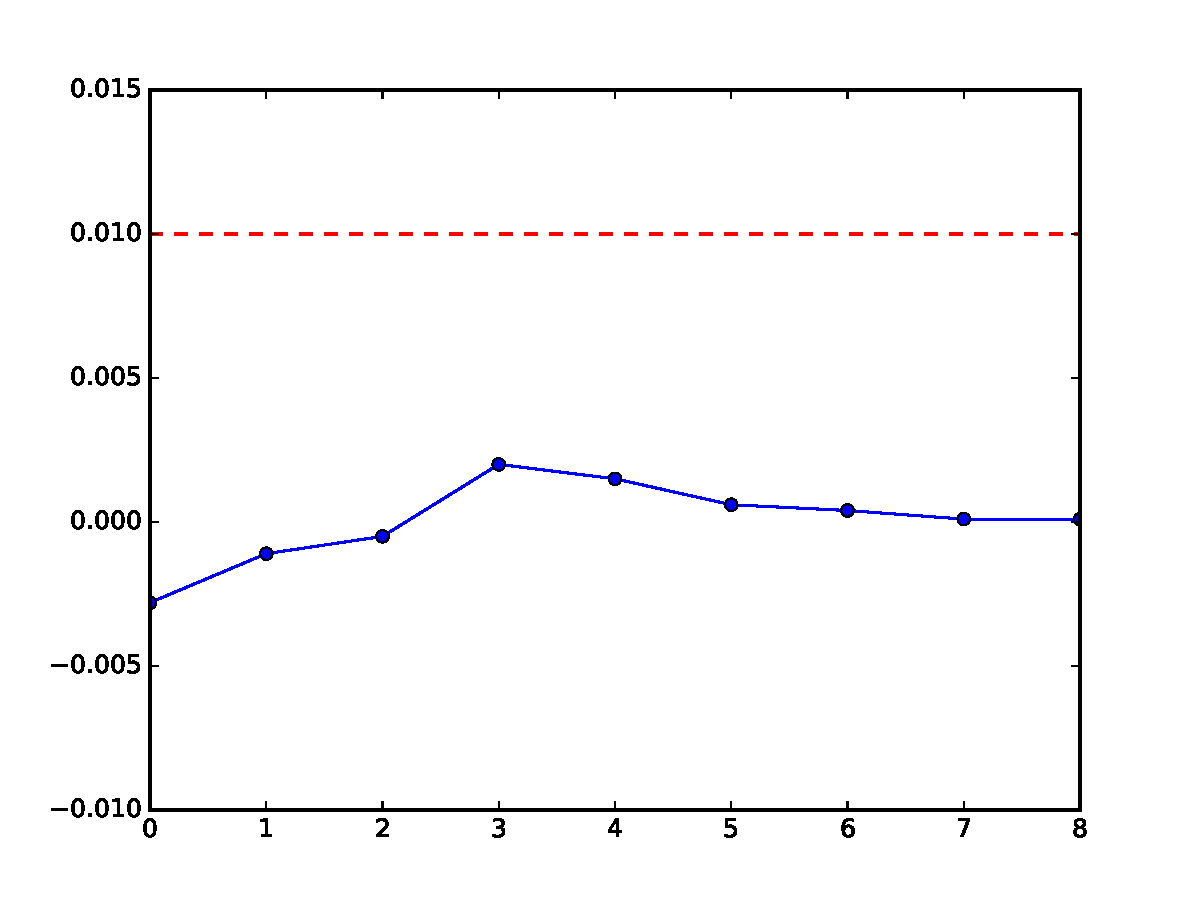
\includegraphics[width=1.0\linewidth]{bandgapDiff.pdf}
				\caption{Difference in the bandgap energies in eV}
				\label{fig:subim2}
			\end{subfigure}
			
			\caption{Here are plots of the differences in relative energies and pressures simulations with different cut-off limits. The difference is found by comparing two different simulations separated by 50ev in the cut-off. The force is safely within the limits of the weak requirement but the strong requirement (sometimes needed e.g. when including phonons) excludes many of the points. For the bandgap, it seems to be well within limits as well}
			\label{fig:image2}
		\end{center}
	\end{figure}
	\newpage
  \subsection{results 1}
  Here are the results for the first simulation
  \lstinputlisting{results.txt}
  \subsection{results 2}
	We often want to compare one structure with itself including some minor adjustment, for example shifting one atom location, because relative measures are much more enlightening than the absolutes. Doing this we can tell a lot more about how the structure behaves. Results 2 are from changing the position of the first Si atoms y-coordinate from 0.0 to 0.02 Ångstrøm.
  \lstinputlisting{results2.txt}
  \subsection{results 3}
	Sometimes we also care about the convergence with respect to the k point density. In these simulations we let the k-point density vary from 1 to 6. The results was as follows.
  \lstinputlisting{results3.txt}
	
  \subsection{python code}
  \lstinputlisting[python]{results.py}
 
  
\end{document}
